\chapter{Моделирование и оценивание}
\label{ch:chap4}

Для оценки эффективности разработанной системы проведем эксперименты при различных сценариях с двумя системами: стандартная система для Nav2 и предложенная система с подсистемой контроля и подсистемой учета динамических объектов.

Эксперименты разделены на 2 части: первая часть нацелена на проверку поведений при различных неполадках (проверка системы контроля), а вторая будет проводиться в условиях динамического окружения (проверка системы учета динамический объектов).

\section{Модификация модели мобильного робота}

Как уже отмечалось в главе 2.3 в качестве мобильного робота был выбран робот ROBOTIS Turtlebot3.

В рамках данной работы в конфигурации робота были внесены следующие изменения:
\begin{enumerate}
    \item Убран модель камеры
    \item Добавлен датчик, реагирующий на столкновения (bumper sensor). Он имеет размеры $10\times265\times25$ мм и прикреплен к передней части робота
\end{enumerate}

\begin{figure}[H]
    \centering
    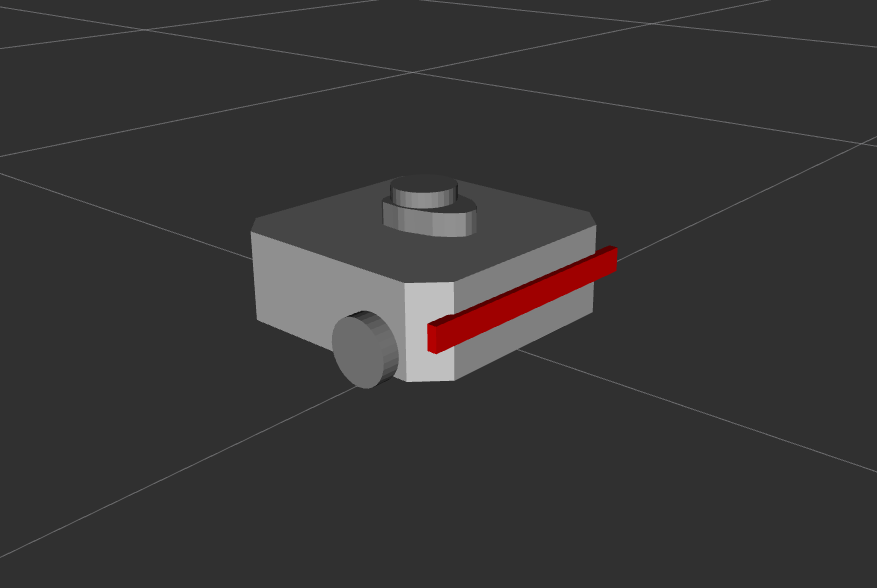
\includegraphics{images/chap_4/tb3-rviz.png}
    \caption{Модель мобильного робота в Rviz (красным цветом отмечен датчик столкновения)}
    \label{fig:tb3-rviz}
\end{figure}

\section{Симуляционные миры}

Эксперименты проводятся в двух окружениях:
\begin{enumerate}
    \item \textit{TurtleBot3 House} - статическое окружение, описывающее модель дома. Эта карта поставляется вместе с пакетом \textit{turtlebot3}. Эксперименты на данной карте будут проводиться для тестирования системы контроля
\begin{figure}[H]
    \centering
    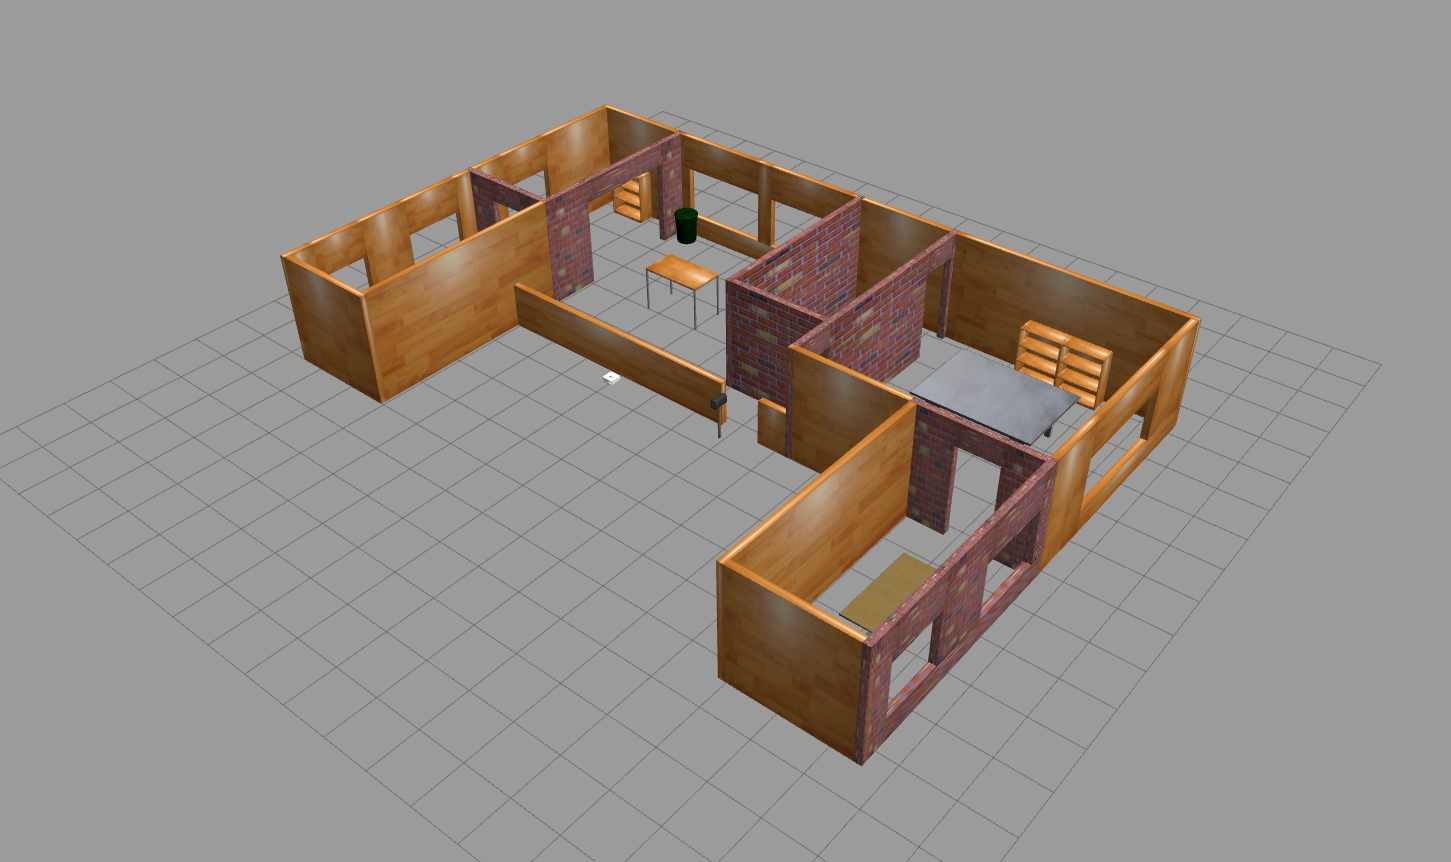
\includegraphics{images/chap_4/tb3-house.png}
    \caption{Симуляционный мир \textit{TurtleBot3 House}}
    \label{fig:tb3-house}
\end{figure}
    \item \textit{Dynamic World} - динамическое окружение, описываюшее замкнутое пространтсво, окруженное стенами высотой $1.5$ м и периметром $5\times10$ м. Внутри пространства находятся 3 пешехода (actors), которые имеют траектории движения параллельно короткой стороне прямоугольника. При тестировании различных сценариев значения скоростей пешеходов будет изменяться, также начальная точка движения пешеходов будет различна при каждом сценарии. Высота пешеходов равна $2$ м, а максимальные размеры на плоскости $XY$ не превышают $30\times30$ см. Эксперименты на данной карте будут проводиться для тестирования системы учета динамических объектов
\begin{figure}[H]
    \centering
    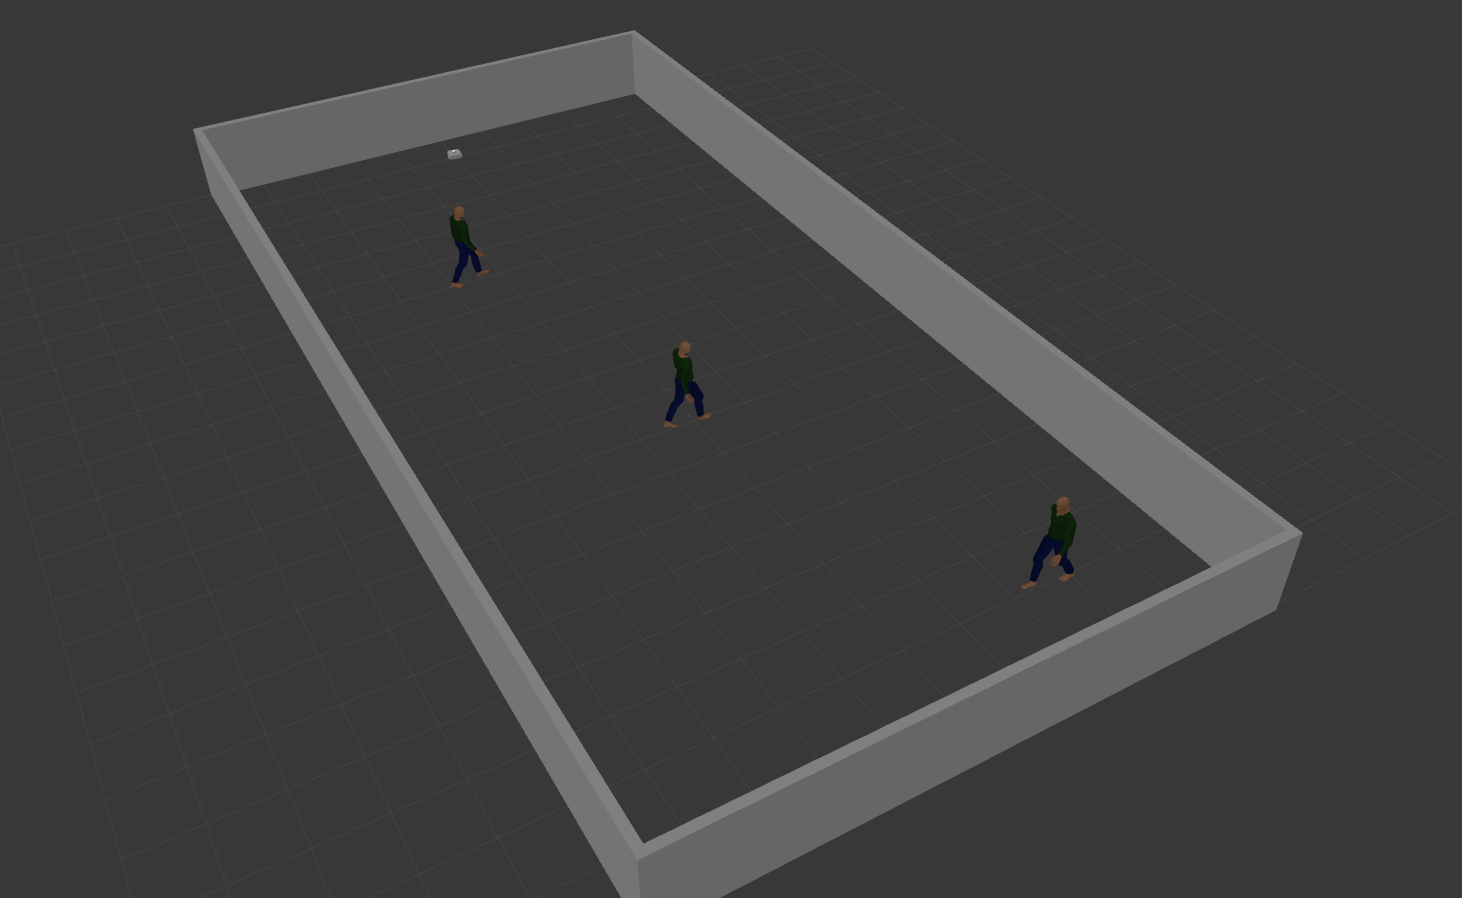
\includegraphics{images/chap_4/dyn-world.png}
    \caption{Симуляционный мир \textit{Dynamic World}}
    \label{fig:dyn-world}
\end{figure}
\end{enumerate}

\section{Картографирование местности}

Для построения статической карты местности и дальнейшей передачи на вход системе навигации использовался SLAM. Таким образом, построенная заранее карта будет использоваться для всех последующих на ней тестов. Это убирает неоходимость "изучения" мобильным роботом окружения при каждом новом запуске.

В частности, в качестве метода SLAM по умолчанию использовался картограф - проект Google с открытым исходным кодом, реализованный в пакете \textit{turtlebot3\_cartographer}. Для выполнения SLAM для обоих вышеупомянутых окружений были созданы две статические карты занятости.

\begin{figure}[H]
    \centering
    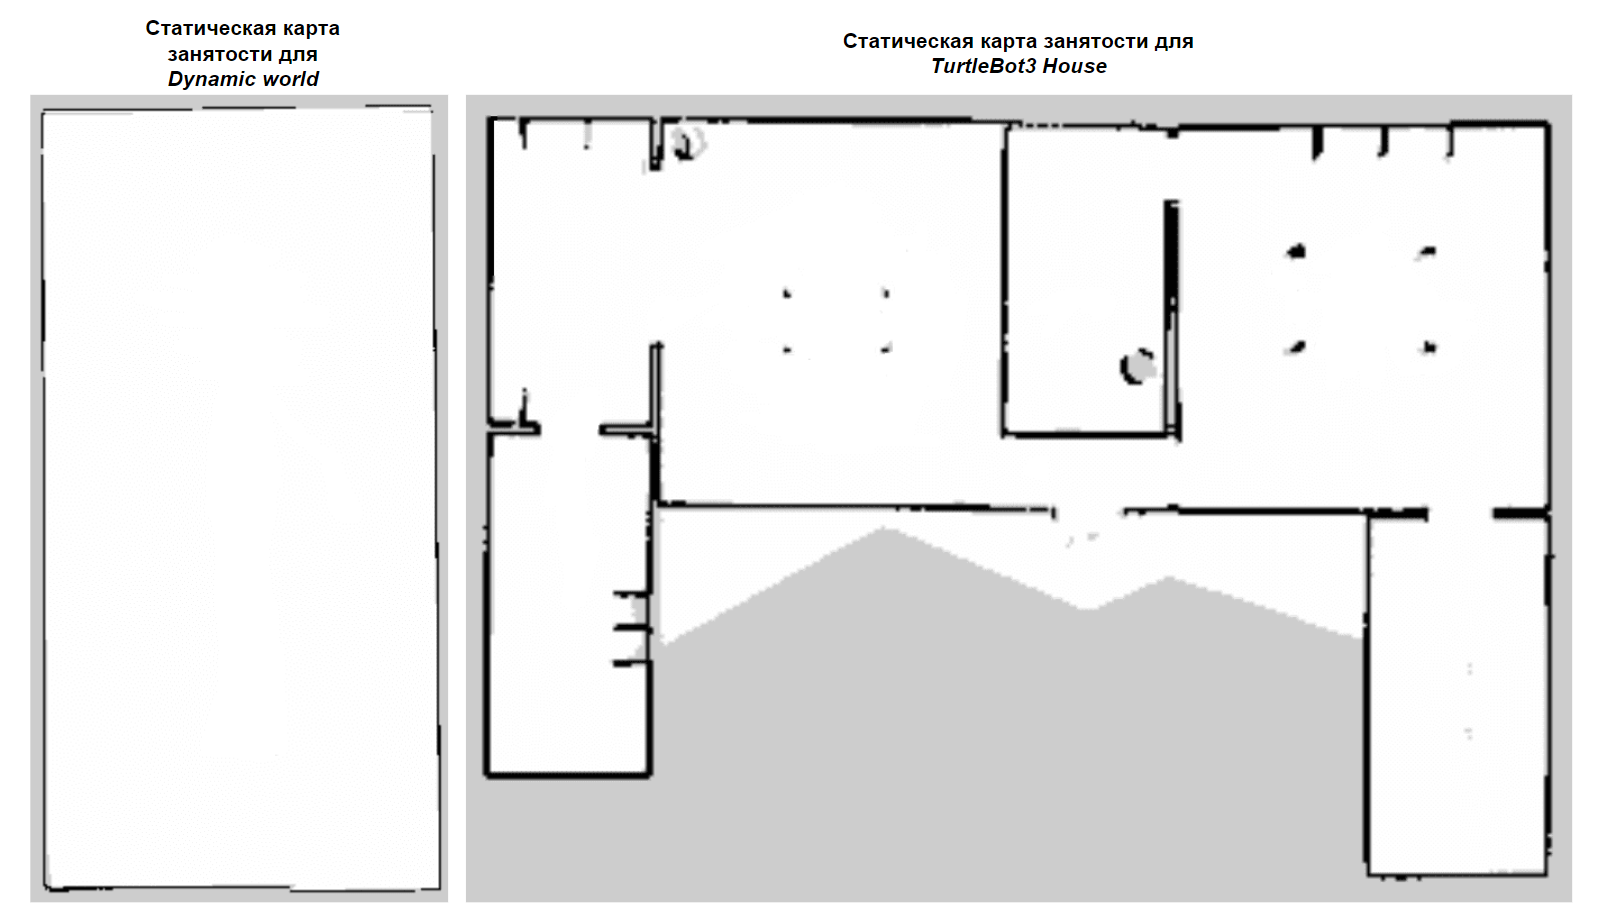
\includegraphics{images/chap_4/oc-grids.png}
    \caption{Статические карты занятости для используемых окружений (масштабы карт изменены)}
    \label{fig:oc-grids}
\end{figure}

\section{Тестирование}

Целью тестирования является получение оценки работоспособности и эффективности разработанной системы и её сравнение с существующими решениями.

Предлагаемые ниже тесты предназначены для сравнения поведения робота в условиях внезапных неполадок с различными компонентами системы и в условиях динамического окружения. 

В тестировании участвуют две системы:
\begin{enumerate}
    \item Стандартная система Nav2. Архитектура представлена на Рисунке \ref*{fig:sys_arch_nav2}. Для удобства дадим ей обозначение \textit{STD}
    \item Cистема Nav2 с внедрением разработанной системы принятия решений. Архитектура представлена на Рисунке \ref*{fig:full-system}. Обозначим её \textit{DMS}
\end{enumerate}

\subsection{Тестирование системы контроля}

\subsubsection{Сценарии}

В Таблицах \ref*{tab:scenarios1} и \ref*{tab:scenarios2} представлены описания сценариев тестирования вместе с критериями успешной отработки данного сценария. Для того чтобы тест был признан успешным, должны быть выполнены все критерии успешной отработки для данного сценария.

\begin{table}[]
\resizebox{\textwidth}{!}{%
\begin{tabular}{|c|l|l|l|}
\hline
\textbf{\begin{tabular}[c]{@{}c@{}}Тестируемый\\ компонент\end{tabular}} & \multicolumn{1}{c|}{\textbf{\begin{tabular}[c]{@{}c@{}}Имя\\ теста\end{tabular}}} & \multicolumn{1}{c|}{\textbf{Описание сценария}}                                                                                                        & \multicolumn{1}{c|}{\textbf{\begin{tabular}[c]{@{}c@{}}Критерии \\ успешной отработки\end{tabular}}} \\ \hline
\multirow{3}{*}{LIDAR}                                                   & \textit{lidar\_1}                                                                 & \begin{tabular}[c]{@{}l@{}}1. Робот стоит\\ 2. Неполадка с LIDAR\end{tabular}                                                                          & 1. Перезапуск LIDAR                                                                                  \\ \cline{2-4} 
                                                                         & \textit{lidar\_2}                                                                 & \begin{tabular}[c]{@{}l@{}}1. Робот двигается \\ с линейной скоростью 0.25 м/с\\ прямо к цели\\ 2. Неполадка с LIDAR\end{tabular}                      & \begin{tabular}[c]{@{}l@{}}1. Перезапуск LIDAR\\ 2. Достижение цели\end{tabular}                     \\ \cline{2-4} 
                                                                         & \textit{lidar\_3}                                                                 & \begin{tabular}[c]{@{}l@{}}1. Робот двигается \\ с линейной скоростью 0.25 м/с\\ и угловой скоростью 0.5 рад/с\\ 2. Неполадка с LIDAR\end{tabular}     & \begin{tabular}[c]{@{}l@{}}1. Перезапуск LIDAR\\ 2. Достижение цели\end{tabular}                     \\ \hline
\multirow{3}{*}{IMU}                                                     & \textit{imu\_1}                                                                   & \begin{tabular}[c]{@{}l@{}}1. Робот стоит\\ 2. Неполадка с LIDAR\end{tabular}                                                                          & 1. Перезапуск IMU                                                                                    \\ \cline{2-4} 
                                                                         & \textit{imu\_2}                                                                   & \begin{tabular}[c]{@{}l@{}}1. Робот двигается\\ с линейной скоростью 0.25 м/с\\ прямо к цели\\ 2. Неполадка с IMU\end{tabular}                         & \begin{tabular}[c]{@{}l@{}}1. Перезапуск IMU\\ 2. Достижение цели\end{tabular}                       \\ \cline{2-4} 
                                                                         & \textit{imu\_3}                                                                   & \begin{tabular}[c]{@{}l@{}}1. Робот двигается\\ с линейной скоростью 0.25 м/с\\ и угловой скоростью 0.5 рад/с\\ 2. Неполадка с IMU\end{tabular}        & \begin{tabular}[c]{@{}l@{}}1. Перезапуск IMU\\ 2. Достижение цели\end{tabular}                       \\ \hline
\multirow{3}{*}{Одометрия}                                               & \textit{odom\_1}                                                                  & \begin{tabular}[c]{@{}l@{}}1. Робот стоит\\ 2. Неполадка с одометрией\end{tabular}                                                                     & 1. Перезапуск одометрии                                                                              \\ \cline{2-4} 
                                                                         & \textit{odom\_2}                                                                  & \begin{tabular}[c]{@{}l@{}}1. Робот двигается\\ с линейной скоростью 0.25 м/с\\ прямо к цели\\ 2. Неполадка с одометрией\end{tabular}                  & \begin{tabular}[c]{@{}l@{}}1. Перезапуск одометрии\\ 2. Достижение цели\end{tabular}                 \\ \cline{2-4} 
                                                                         & \textit{odom\_3}                                                                  & \begin{tabular}[c]{@{}l@{}}1. Робот двигается\\ с линейной скоростью 0.25 м/с\\ и угловой скоростью 0.5 рад/с\\ 2. Неполадка с одометрией\end{tabular} & \begin{tabular}[c]{@{}l@{}}1. Перезапуск одометрии\\ 2. Достижение цели\end{tabular}                 \\ \hline
\end{tabular}}
\caption{Таблица сценариев для тестирования датчиков LIDAR и IMU, а также одометрии}
\label{tab:scenarios1}
\end{table}

% Please add the following required packages to your document preamble:
% \usepackage{multirow}
\begin{table}[]
\resizebox{\textwidth}{!}{%
\begin{tabular}{|c|l|l|l|}
\hline
\textbf{\begin{tabular}[c]{@{}c@{}}Тестируемый\\ компонент\end{tabular}} & \multicolumn{1}{c|}{\textbf{\begin{tabular}[c]{@{}c@{}}Имя\\ теста\end{tabular}}} & \multicolumn{1}{c|}{\textbf{Описание сценария}}                                                                                                     & \multicolumn{1}{c|}{\textbf{\begin{tabular}[c]{@{}c@{}}Критерии \\ успешной отработки\end{tabular}}}                                                                                                                          \\ \hline
\multirow{2}{*}{Столкновение}                                            & collision\_1                                                                      & \begin{tabular}[c]{@{}l@{}}1. Робот стоит\\ 2. Произошло столкновение\end{tabular}                                                                  & \begin{tabular}[c]{@{}l@{}}1. Отмена навигации\\ 2. Ожидание выхода из\\ состояния столкновения\\ 3. Добавление объекта\\ столкновения на карту\\ 4. Провека всех \\ компонент системы\end{tabular}                           \\ \cline{2-4} 
                                                                         & collisioin\_2                                                                     & \begin{tabular}[c]{@{}l@{}}1. Робот двигается\\ с линейной скоростью 0.25 м/с\\ 2. Произошло столкновение\\ с недетектируемым объектом\end{tabular} & \begin{tabular}[c]{@{}l@{}}1. Отмена навигации\\ 2. Ожидание выхода из\\ состояния слокновения\\ 3. Добавление объекта\\ столкновения на карту\\ 4. Провека всех \\ компонент системы\\ 5. Продолжение навигации\end{tabular} \\ \hline
Батарея                                                                  & battery\_1                                                                        & \begin{tabular}[c]{@{}l@{}}1. Уровень заряда батареи \\ недостаточен для достижения цели\end{tabular}                                               & \begin{tabular}[c]{@{}l@{}}1. Робот не будет двигаться\\ к цели, которая находится\\ за пределами\end{tabular}                                                                                                                \\ \hline
\begin{tabular}[c]{@{}c@{}}Глобальный\\ планировщик\end{tabular}         & gl\_pl\_1                                                                         & \begin{tabular}[c]{@{}l@{}}1. Робот стоит\\ 2. Путь до цели не может быть\\ вычислен\end{tabular}                                                   & \begin{tabular}[c]{@{}l@{}}1. Перезапустить\\ глобальный планировщик\\ 2. Перестроить путь\\ до цели\\ 3. Достигнуть цель\end{tabular}                                                                                        \\ \hline
\end{tabular}}
\caption{Таблица сценариев для тестирования глобального планировщика, столкновений и недостаточного уровня заряда батареи}
\label{tab:scenarios2}
\end{table}

В тестах с LIDAR, IMU и одометрией драйвер датчика отключался при достижении желаемой скорости, указанной в описании сценария. Каждый из данных компонент был протестирован несколько раз в трех различных ситуациях навигации.

В сценарии \textit{collision\_1} столкновение регистрируется датчиком столкновения. Данный сценарий проверяет способность системы контроля проверять состояние робота после столкновения, обновлять карту местности и возобновлять навигацию. 

\textit{collision\_2} тестирует то же поведение, однако теперь робот находится в процессе навигации. На пути робота возникает недетектируемое препятствие, оно находится слишком низко, чтобы его мог обнаружить датчик LIDAR. Робот должен способен восстановиться после столкновения и продолжить движение к цели по обновленному пути.

Сценарий \textit{battery\_1} проверяет поведение робота при низком заряде батареи. Симулируемая батарея разряжается до низкого уровня, и задается новая цель навигации. Тест завершается неудачей, если во время навигации заряд батареи опускается ниже нуля процентов.

\textit{gl\_pl\_1} - сценарий, в котором состояние жизненного цикла глобального планировщика переходит в "неактивное" и не может больше выполнять действия по планированию при срабатывании. В этом случае модуль основного поведенческого дерева должен обработать данное событие и восстановить функционирование навигации. 

\subsubsection{Результаты}

Результаты, приведенные в Таблице \ref*{tab:results1}, свидетельствуют о существенном увеличении процента успешного выполнения тестовых сценариев разработанной системы. Система контроля достаточно надежна в предложенных сценариях и позволяет системе восстанавливаться после неожиданной неисправности какой-то компоненты. 

Сценарий недостаточного уровня заряда батареи был успешным каждый раз, когда проводилось тестирование. \\
Однако поведение планирования пути для перезапуска планировщика успешно выполнялось не всегда (90\%). \\
Поведение при столкновениях работает достаточно хорошо и одним из важным компоненом этого является обновление карты местности для добавления объекта столкновения на нее. Тем не менее, в 30-40\% случаев роботу не хватает автономности продолжить выполнение задач после столкновения. 

В результате проведенного тестирования можно выделить следующие функциональные особенности, которые превнесла реализованная система контроля в уже существующую архитектуру:
\begin{enumerate}
    \item Система обнаруживает сбой компоненты. В таких ситуациях система может перезапускать датчики и снижать скорость в течение некоторого времени, когда компонент предоставляет ограниченную информацию
    \item Система обнаруживает аварийные ситуации. Cистема может обнаружить, когда продолжение движения по рассчитанному пути уже небезопасно (отказ датчиков, нехватка заряда батареи, блокирование объектом)
    \item Система может инициировать аварийную остановку. Система может отменить все команды и остановиться в случае обнаружения аварийной ситуации
    \item Система может отменить команды с Nav2. Команды системы всегда могут отменить команды, поступающие от Nav2
    \item Система предотвращает случаи, когда во время движения к цели у робота разрядится аккумулятор
    \item (Выполняется не всегда) Система может восстанавливаться после столкновений
\end{enumerate}

Также помимо приведенных выше функциональных преимуществ, разработанная система обладает некоторыми архитектурными особенностями. Отметим наиболее важные из них:
\begin{enumerate}
    \item Архитектурный дизайн системы контроля устраняет единую точку отказа системы. Даже если система Nav2 станет недоступна во время движения, робот сможет корректно обработать данный сценарий и безопасно приостановить навигацию
    \item Производительность системы при проверке условий основного поведенческого дерева достаточна для успешного выполнения задач навигации в динамическом окружении. Этого удалось достичь за счет применения принципа модульности при реализации (вся система работает в нескольких потоках)
\end{enumerate}

\begin{table}[]
\centering
\begin{tabular}{|l|l|ll|}
\hline
\multicolumn{1}{|c|}{\multirow{2}{*}{\textbf{Имя теста}}} & \multicolumn{1}{c|}{\multirow{2}{*}{\textbf{\begin{tabular}[c]{@{}c@{}}Количество\\ симуляций\end{tabular}}}} & \multicolumn{2}{c|}{\textbf{Процент успеха, \%}}                      \\ \cline{3-4} 
\multicolumn{1}{|c|}{}                                    & \multicolumn{1}{c|}{}                                                                                        & \multicolumn{1}{c|}{\textbf{STD}} & \multicolumn{1}{c|}{\textbf{DMS}} \\ \hline
\textit{lidar\_1}                                         & 5                                                                                                            & \multicolumn{1}{l|}{0}            & 100                               \\ \hline
\textit{lidar\_2}                                         & 5                                                                                                            & \multicolumn{1}{l|}{0}            & 100                               \\ \hline
\textit{lidar\_3}                                         & 5                                                                                                            & \multicolumn{1}{l|}{0}            & 100                               \\ \hline
\textit{imu\_1}                                           & 5                                                                                                            & \multicolumn{1}{l|}{0}            & 100                               \\ \hline
\textit{imu\_2}                                           & 5                                                                                                            & \multicolumn{1}{l|}{0}            & 100                               \\ \hline
\textit{imu\_3}                                           & 5                                                                                                            & \multicolumn{1}{l|}{0}            & 100                               \\ \hline
\textit{odom\_1}                                          & 5                                                                                                            & \multicolumn{1}{l|}{0}            & 100                               \\ \hline
\textit{odom\_2}                                          & 5                                                                                                            & \multicolumn{1}{l|}{0}            & 100                               \\ \hline
\textit{odom\_3}                                          & 5                                                                                                            & \multicolumn{1}{l|}{0}            & 100                               \\ \hline
\textit{collision\_1}                                     & 10                                                                                                           & \multicolumn{1}{l|}{0}            & 80                                \\ \hline
\textit{collision\_2}                                     & 10                                                                                                           & \multicolumn{1}{l|}{0}            & 60                                \\ \hline
\textit{battery\_1}                                       & 10                                                                                                           & \multicolumn{1}{l|}{0}            & 100                               \\ \hline
\textit{gl\_pl\_1}                                        & 10                                                                                                           & \multicolumn{1}{l|}{0}            & 90                                \\ \hline
\end{tabular}
\caption{Результаты тестирования системы контроля}
\label{tab:results1}
\end{table}

\subsection{Тестирование системы учета динамических объектов}

Для тестирования работы системы в условиях динамического окружения будем использовать мир \textit{Dynamic World} с различными конфигурациями движущихся объектов. 

Стоит отметить, что каждый динамический объект в окружении (пешеход) симуляции был создан с использованием плагина \textit{actor\_collisions} \cite{actor-coll}. Добавление этого плагина позволяет пешеходу иметь свойства столкновения (\textit{<collision>}), что позволяет динамическим пешеходам или препятствиям быть охваченными лидаром в сцене моделирования Gazebo. То есть использование данного плагина увеличивает степень реалистичности моделирования.

\subsubsection{Сценарии}

Для тестирования системы в динамическом окружении были придуманы 3 сценария, отличающихся только значениями скоростей пешеходов, они представлены в Таблице \ref*{tab:scen-dyn-1}.

Все сценарии происходят в окружении \textit{Dynamic World}. Роботу задается цель навигации, расположенная на противополжной стороне прямоугольной зоны. Общее расстояние пути равно $8$ метрам. Упрощенная схема тестирования изображена на Рисунке \ref*{fig:test-scheme}. \\

% figure
\begin{figure}[H]
    \centering
    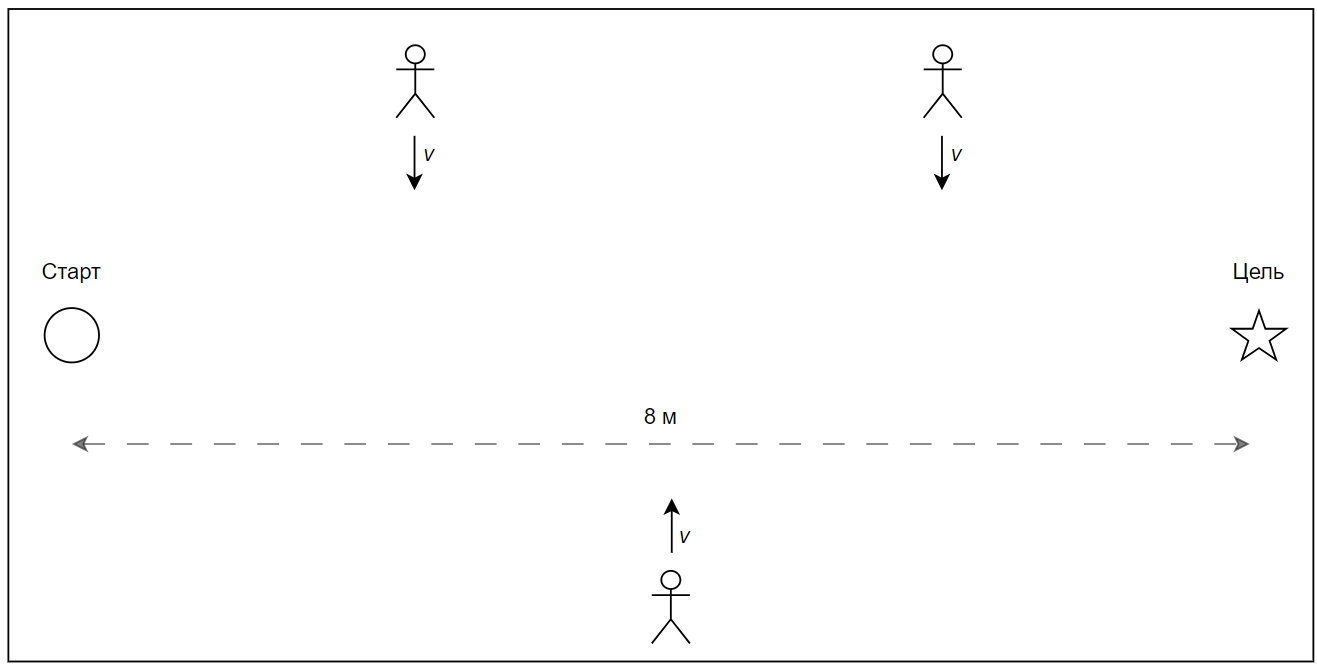
\includegraphics[width=0.75\textwidth]{images/chap_4/test-scheme.png}
    \caption{Упрощенная схема тестирования в условиях динамических объектов}
    \label{fig:test-scheme}
\end{figure}

Для оценивания рассчитываются три величины: 
\begin{enumerate}
    \item Успешная навигация - процент от общего числа тестов, при котором робот достигает цель навигации
    \item Поведение ожидания - это процент от общего числа тестов, во время которых срабатывало поведение ожидания (\textit{wait}), но при этом цель навигации была достигнута. Поведение ожидания вызывается сервером восстановления, когда препятствия внезапно оказываются слишком близко и сервер управления не может найти приемлемый путь в течение некоторого времени
    \item Столкновение - процент от общего числа тестов, в которых не была достигнута цель навигации из-за столкновения робота с пешеходом

\end{enumerate}

% table
\begin{table}[H]
\centering
\begin{tabular}{|c|c|}
\hline
\textbf{Номер теста} & \textbf{Скорость пешеходов, м/с} \\ \hline
1                    & \textit{0.5}                     \\ \hline
2                    & \textit{0.75}                    \\ \hline
3                    & \textit{1.0}                     \\ \hline
\end{tabular}
\caption{Таблица с данными о скоростях пешеходов при тестировании}
\label{tab:scen-dyn-1}
\end{table}

\subsubsection{Результаты}

Для каждого из трех сценариев тестирование проводилось 25 раз.\\
Результаты каждого эксперимента для двух систем представлены в Таблице \ref*{tab:results-dyn}.

\begin{table}[H]
\centering
\begin{tabular}{c|cc|cc|cc|}
\cline{2-7}
\textbf{}                                                                            & \multicolumn{2}{c|}{\textbf{\begin{tabular}[c]{@{}c@{}}Успешная\\ навигация,\\ \%\end{tabular}}} & \multicolumn{2}{c|}{\textbf{\begin{tabular}[c]{@{}c@{}}Поведение\\ ожидания,\\ \%\end{tabular}}} & \multicolumn{2}{c|}{\textbf{\begin{tabular}[c]{@{}c@{}}Столкновение,\\ \%\end{tabular}}} \\ \hline
\multicolumn{1}{|c|}{\textbf{\begin{tabular}[c]{@{}c@{}}Номер\\ теста\end{tabular}}} & \multicolumn{1}{c|}{STD}                                  & DMS                                  & \multicolumn{1}{c|}{STD}                                  & DMS                                  & \multicolumn{1}{c|}{STD}                              & DMS                              \\ \hline
\multicolumn{1}{|c|}{1}                                                              & \multicolumn{1}{c|}{\textit{96}}                          & \textit{100}                         & \multicolumn{1}{c|}{\textit{0}}                           & \textit{8}                           & \multicolumn{1}{c|}{\textit{4}}                       & \textit{0}                       \\ \hline
\multicolumn{1}{|c|}{2}                                                              & \multicolumn{1}{c|}{\textit{64}}                          & \textit{72}                          & \multicolumn{1}{c|}{\textit{0}}                           & \textit{28}                          & \multicolumn{1}{c|}{\textit{36}}                      & \textit{28}                      \\ \hline
\multicolumn{1}{|c|}{3}                                                              & \multicolumn{1}{c|}{\textit{28}}                          & \textit{48}                          & \multicolumn{1}{c|}{\textit{0}}                           & \textit{44}                          & \multicolumn{1}{c|}{\textit{72}}                      & \textit{52}                      \\ \hline
\end{tabular}
\caption{Результаты тестирования системы в динамическом окружении}
\label{tab:results-dyn}
\end{table}

Анализируя результаты, можно увидеть, что разработанная система учета динамических объектов показала более высокий процент успешной навигации во всех 3-х сценариях. Наиболее существенное улучшение происходит на третьем тесте (скорость пешеходов $1$ м/с).

Также разработанная система меньше попадает в столкновения с объектами. Это напрямую связано с увеличением процента поведения ожидания. Ведь с добавлением слоя для локального планировщика, в котором отмечена зона вокруг динамических объектов в форме гауссовкого распределения - это позволяет учитывать величину и направление движения объектов мобильным роботом. А значит что сервер восстановления срабатывает своевременно и вызывает поведение ожидания, а значит удаётся предотвратить столкновение. 
